\RequirePackage[l2tabu,orthodox]{nag}
\documentclass[usenames,dvipsnames,compress]{beamer}
\usepackage[english,russian]{babel}
\usepackage{polyglossia}
\setmainlanguage{russian}

% \usepackage[T2A]{fontenc}
\usepackage[OT2, T1]{fontenc}
\usepackage[utf8]{inputenc}
% \usepackage[english,russian]{babel}

\usepackage{newtxtext}
\usepackage{newtxmath}
\usepackage{microtype}
\usepackage{hyperref}
\usepackage{tabu}
\usepackage{csquotes}
\usepackage{underscore}


\usepackage{listings}
\lstset{language=C,basicstyle=\ttfamily,columns=flexible,showstringspaces=false}

\lstdefinelanguage{diff}{
  basicstyle=\ttfamily\small,
  morecomment=[f][\color{Gray}]{@@},
  morecomment=[f][\color{Green}]{+\ },
  morecomment=[f][\color{OrangeRed}]{-\ },
}

\hypersetup{
  colorlinks=true,
  urlcolor=CadetBlue, % MidnightBlue,
  linkcolor=CadetBlue, % MidnightBlue,
}

\newcommand \T[1]{\texttt{#1}}

\usepackage{tikz}
\usepackage{diagbox}

% \usefonttheme{professionalfonts}


\setbeamertemplate{footline}[page number]
\begin{document}
\begin{frame}
  \title{Разработка инструмента для обнаружения состояний гонки времени сборки}
  \author{Vladislav Ivanishin \\ \href{mailto:vlad@ispras.ru}{vlad@ispras.ru}}
  \institute{\includegraphics[height=0.35cm]{\detokenize{logo_EN_basic}}}
  \date{\today{}}
  \titlepage
  \nocite{*} % Show bibliography references even if they are not cited
\end{frame}

\begin{frame}[fragile]{Makefile (race condition demo)}
\begin{lstlisting}[language=make]
# Should actually depend on prog.c *and common.c*
prog: prog.c
        gcc prog.c common.c -o prog

# Making this target will result in making common.c first
libcommon.so: common.c
        gcc -shared common.c -o libcommon.so

# common.c is generated in some way based on common.in
common.c: common.in
        ln common.in common.c
\end{lstlisting}

\hfill

\tt{make -j2 all}

will have different results...
\end{frame}

\begin{frame}[fragile]{Dependency graph}
\includegraphics[scale=0.75]{demo}
\end{frame}


\begin{frame}[fragile]{Gentoo Bugzilla: -j1 hotfixes}
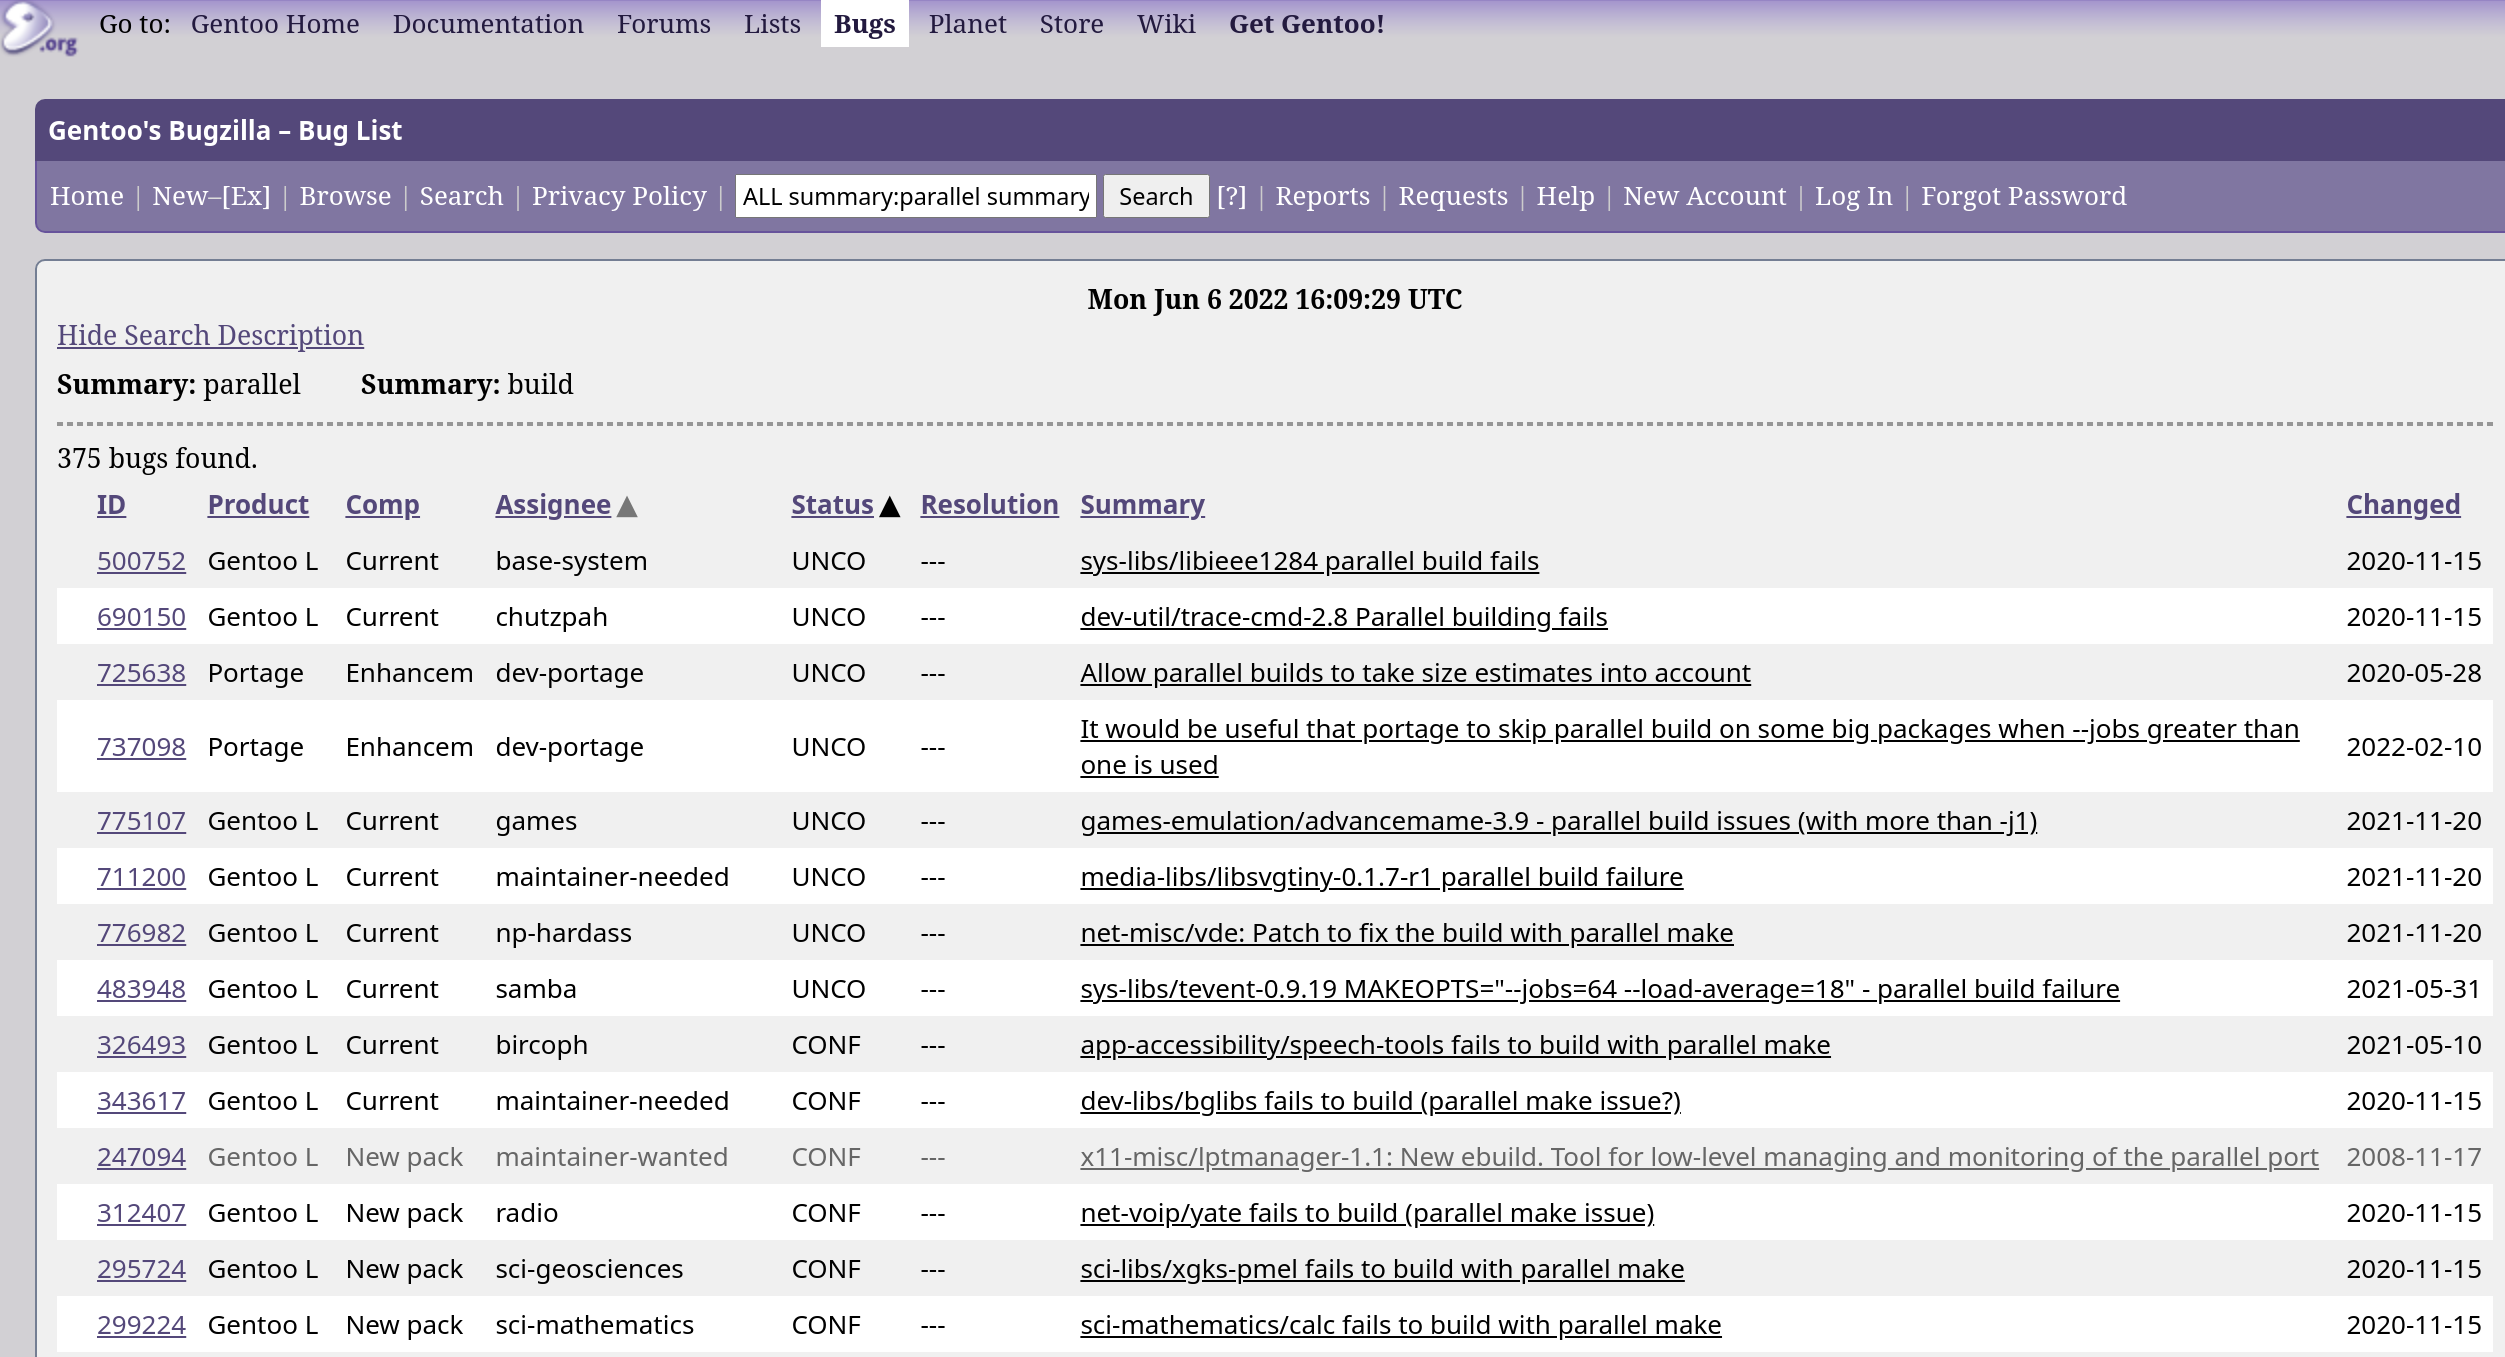
\includegraphics[scale=0.15]{bugzilla}
\end{frame}

\end{document}
